\scnheader{Введение в язык графического представления баз знаний ostis-систем}
\scnidtf{Введение в SCg-код}
\scnreltovector{конкатенация сегментов}{Первый сегмент Введения в SCg-код;Описание Ядра SCg-кода;Описание Первого расширения Ядра SCg-кода;Описание Второго расширения Ядра SCg-кода;Описание Третьего расширения Ядра SCg-кода;Описание Четвертого расширения Ядра SCg-кода;Описание Пятого расширения Ядра SCg-кода;Описание Шестого расширения Ядра SCg-кода;Описание Седьмого расширения Ядра SCg-кода;Последний сегмент Введения в SCg-код}

\scnheader{следует отличать*}
\scnhaselement{\scnset{\textit{SCg-код}; \textit{Введение в SCg-код}}}
\scnhaselement{\scnset{\textit{Ядро SCg-кода}; \textit{Описание Ядра SCg-кода}}}
\scnhaselement{\scnset{\textit{Первое расширение Ядра SCg-кода}; \textit{Описание Первого расширения Ядра SCg-кода}}}

\scnsourcecomment{То есть следует отличать саму описываемую сущность и текст, являющийся описанием этой сущности}

\scnheader{SCg-код}
\scnidtf{Semantic Code graphical}
\scnidtf{Язык визуального (графического) представления баз знаний ostis-систем}
\scnexplanation{SCg-код представляет собой способ визуализации sc-текстов (sc-конструкций) в виде рисунков этих конструкций. Подчеркнем, что абстрактная графовая структура и её рисунок (графическое изображение) -- это не одно и тоже даже, они изоморфны друг другу. SCg-код рассматривается нами как \textit{объединение*} нескольких его подъязыков, в число которых входит Ядро SCg-кода, обеспечивающее изоморфное графическое изображение любого sc-текста, а также несколько направлений расширения этого ядра, обеспечивающих повышение компактности и и читабельности текстов SCg-кода (sc.g-текстов, sc.g-конструкций).}

\scnendstruct

\scnsegmentheader{Описание Ядра SCg-кода}

\scnstartsubstruct

\bigskip
\scnfilelong{Алфавиту SC-кода взаимно однозначно соответствует алфавит \textit{Ядра SCg-кода} (алфавит sc.g-элементов, графически изображающих sc-элементы). Все sc-узлы, не являющиеся знаками файлов в тексте (конструкции) \textit{Ядра SCg-кода} изображаются в виде небольших чёрных кругов одинакового радиуса, который обозначим через $r$, и точная величина которого зависит от масштаба отображения sc.g-конструкции. Каждое \uline{sc-ребро} в \textit{Ядре SCg-кода} изображается в виде линии произвольной формы не имеющий самопересечений и имеющей толщину, равную примерно $r/8$.

Каждая \uline{sc-дуга} в \textit{Ядре SCg-кода} изображается в виде линии произвольной формы, не имеющей самопересечений, имеющей толщину равную $r/8$ и имеющей изображение стрелочки на одном из концов этой линии. 

Каждая входящая в sc-конструкцию \uline{базовая sc-дуга} в \textit{Ядре SCg-кода} изображается в виде линии произвольной формы, не имеющий самопересечений, имеющий толщину $r/4$, и имеющей изображение стрелочки на одном из ее концов. 

Каждый входящий в sc-конструкцию \uline{sc-узел}, имеющий содержимое, в \textit{Ядре SCg-кода} изображается в виде прямоугольника произвольного размера с толщиной линии $r/6$. Внутри этого прямоугольника отображается файл, обозначаемый изображаемым sc-узлом. Если нет необходимости изображать в тексте сам файл, обозначаемый sc-узлом, имеющим содержимое, то такой sc-узел в Sc.g-тексте изображается в виде прямоугольника со сторонами $2r$ по вертикали и $4r$ по горизонтали.

Представим таблицу соответствия между \textit{Алфавитом SC-кода} (Алфавитом абстрактных элементов sc-конструкций) и \textit{Алфавитом Ядра SCg-кода} (Алфавитом графических примитивов, составляющих конструкции Ядра SCg-кода и являющихся изображениями sc-элементов).}

\scnheader{Таблица. Алфавит Ядра SCg-кода}
\scneqfile{\\
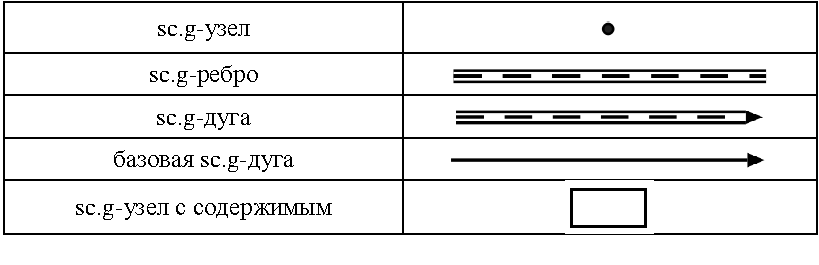
\includegraphics{figures/intro/SCg-core-alphabet.pdf}\\
}

\scnheader{Описание Ядра SCg-кода}
\scnseminclusion{Трудно сразу поверить, что на основе такого простого алфавита можно построить удобный и \uline{универсальный} графовый язык. В рамках \textit{Описания Технологии OSTIS} мы постараемся Вас в этом убедить. Кроме того, нас не должна настораживать простота алфавита, поскольку человечество имеет большой опыт кодирования, хранения в памяти и передачи по каналам связи самых различных информационных ресурсов, используя алфавит, состоящий только из двух классов элементов -- единиц и нулей. 

Мы ведем речь о принципиально ином (графовом) способе кодирования информации в компьютерных системах, но стараемся при этом свести это кодирование к достаточно простому алфавиту хотя бы для того, чтобы искусственно не усложнять проблему создания нового поколения компьютеров, основанных на указанном способе кодирования информации. 

Расширения \textit{Ядра SCg-кода} рассмотрим как направления перехода от текстов \textit{Ядра SCg-кода} к более компактным текстам. Но, поскольку это приводит к усложнению \textit{Синтаксиса SCg-кода} и, в первую очередь, к расширению \textit{Алфавита SCg-кода}, делать такие расширения необходимо обоснованно с учетом частоты встречаемости в рамках \textit{баз знаний ostis-систем} соответствующих фрагментов.}

\scnendstruct